\documentclass[a4paper, 12pt]{article}

\usepackage[portuges]{babel}
\usepackage[utf8]{inputenc}
\usepackage[margin=1.0in]{geometry}
\usepackage{amsmath}
\usepackage{graphicx}
\usepackage{datetime}
\usepackage{enumerate}
\renewcommand{\baselinestretch}{1.5}

\emergencystretch 1pt%

\title{EFC2 - Classificação}
\author{Rafael Gonçalves - RA: 186062}
\date{}

\begin{document}


\maketitle

\section*{Parte I - Teoria Bayesiana de Decisão}

\begin{figure}[h!]
    \centering
    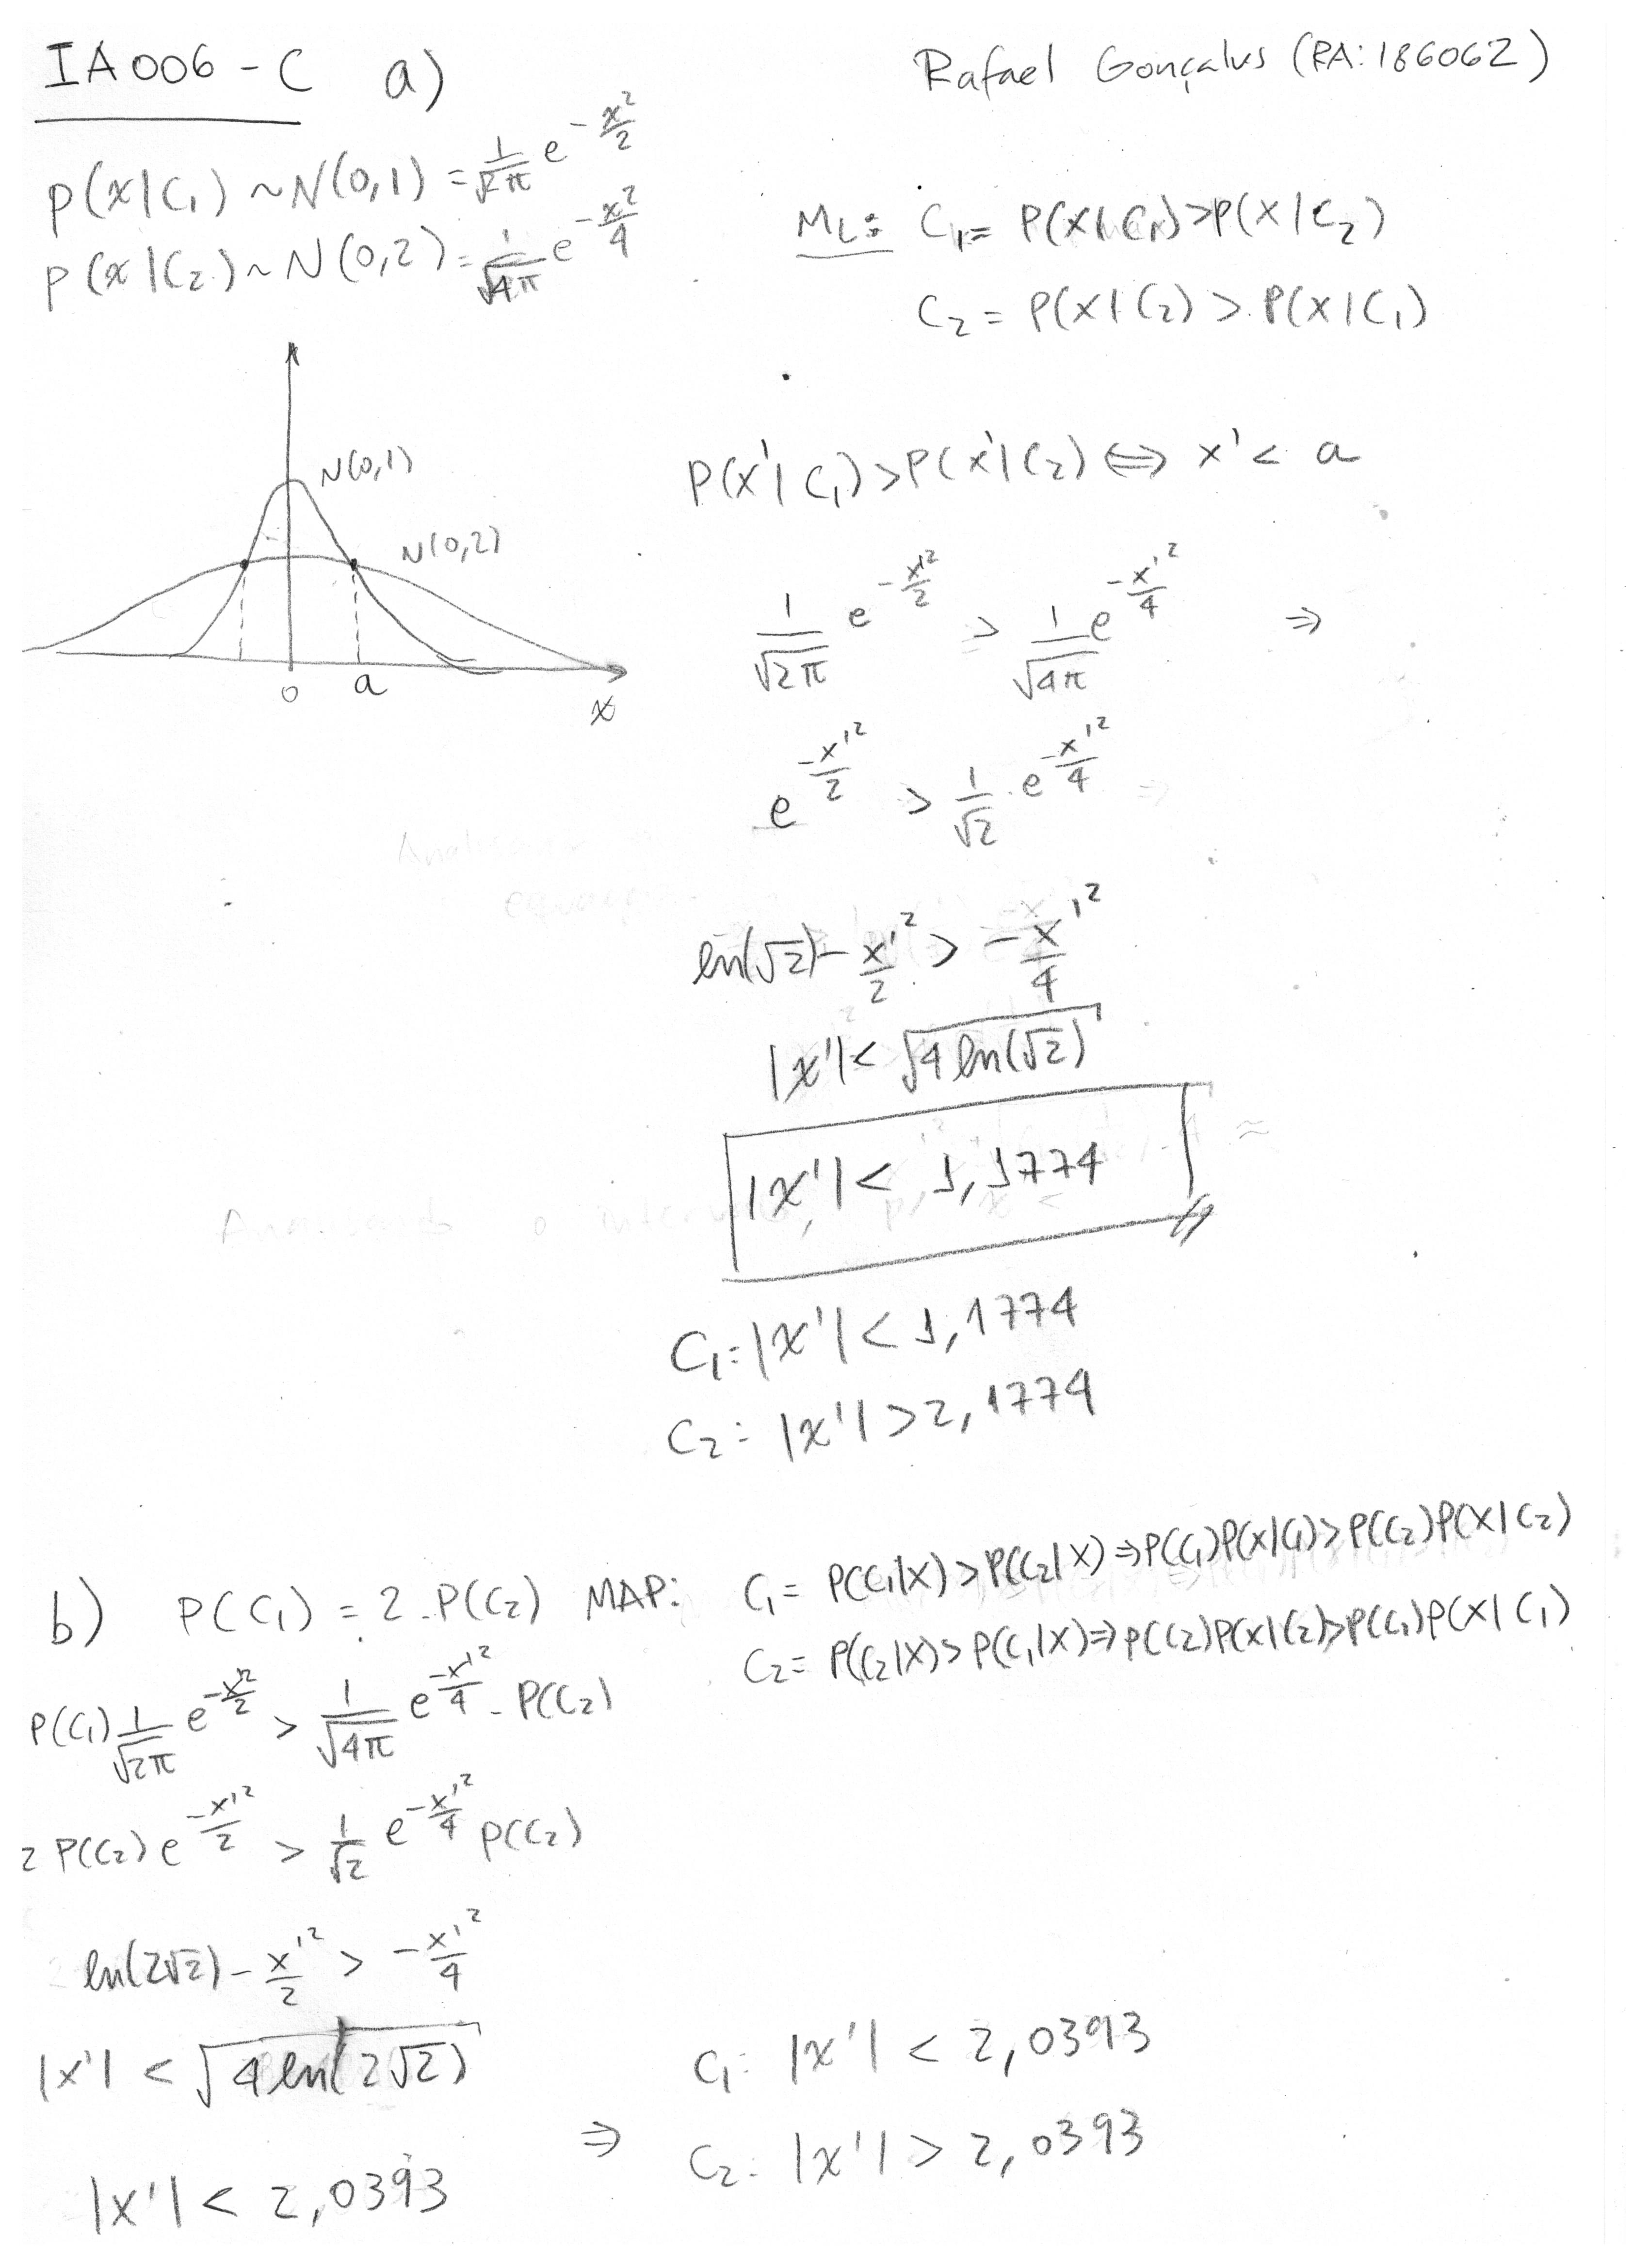
\includegraphics[width=1.0\textwidth]{images/parteI.png}
\end{figure}

\subsection*{c)}

Dado que o critério MAP leva em consideração a probabilidade a posteriori e o critério ML não, os resultados podem ser bem diferentes entre os dois estimadores.

O critério ML diz quão semelhantes são as duas distribuições de probabilidade das classes P(x;Ck).
No caso do exercício, a fronteira de decisão para o caso do estimador ML é basicamente o ponto de intersecção entre o plot das duas distribuições gaussianas - onde a distribuição P(x;C1) é maior que P(x;C2), x pertence a C1, e x pertence a C2 caso contrário.

O critério MAP leva em conta uma segunda distribuição de probabilidade para cada classe, desta vez a probabilidade a posteriori dos dados.
Desta forma o intervalo em que os dados pertencem a C1 e a C2 podem ser bem diferentes para este critério em relação ao critério ML.
No exercício enquanto que a fronteira de decisão do critério ML foi $x = \pm 1.1774$, para o estimador MAP a fronteira foi $x = \pm 2.0393$.


\end{document}
